Un diagramme de Bode est un outil pour l'analyse du comportement fréquentiel de nombreux circuits, utilisé de façon universelle par les ingénieurs électriciens.\\

Il est constitué de 2 éléments :
\begin{enumerate}
	\item Le diagramme en \textbf{amplitude} : Pour un signal sinusoïdal à une fréquence donnée, il donne le rapport d'amplitude du signal de sortie et du signal d'entrée du circuit. Ce rapport d'amplitude est généralement exprimé en décibels (dB), à savoir un rapport de puissances, dont la définition est la suivante : 
	\begin{align*}
		20 \log_{10}\left( \frac{V_{out}}{V_{in}}\right)
	\end{align*}
	\item Le diagramme en \textbf{phase} : Pour un signal sinusoïdal à une fréquence donnée, il donne le déphasage du signal de sortie par rapport au signal d'entrée, exprimé en degrés ou en radians. 
\end{enumerate}
\vspace{.25cm}

Le diagramme de Bode de la Figure \ref{fig3:lpf} donne un exemple de ce que l'on peut observer dans le cas d'un filtre passe-bas. La fréquence de coupure, représentée ici par un trait rouge, est la fréquence à partir de laquelle le filtre commence à atténuer l'amplitude du signal d'entrée. Avant cette fréquence, le signal d'entrée et de sortie ont la même amplitude. Au-delà de cette fréquence, le signal de sortie est atténué par rapport au signal d'entrée.

\begin{figure}[!ht]
	\centering
	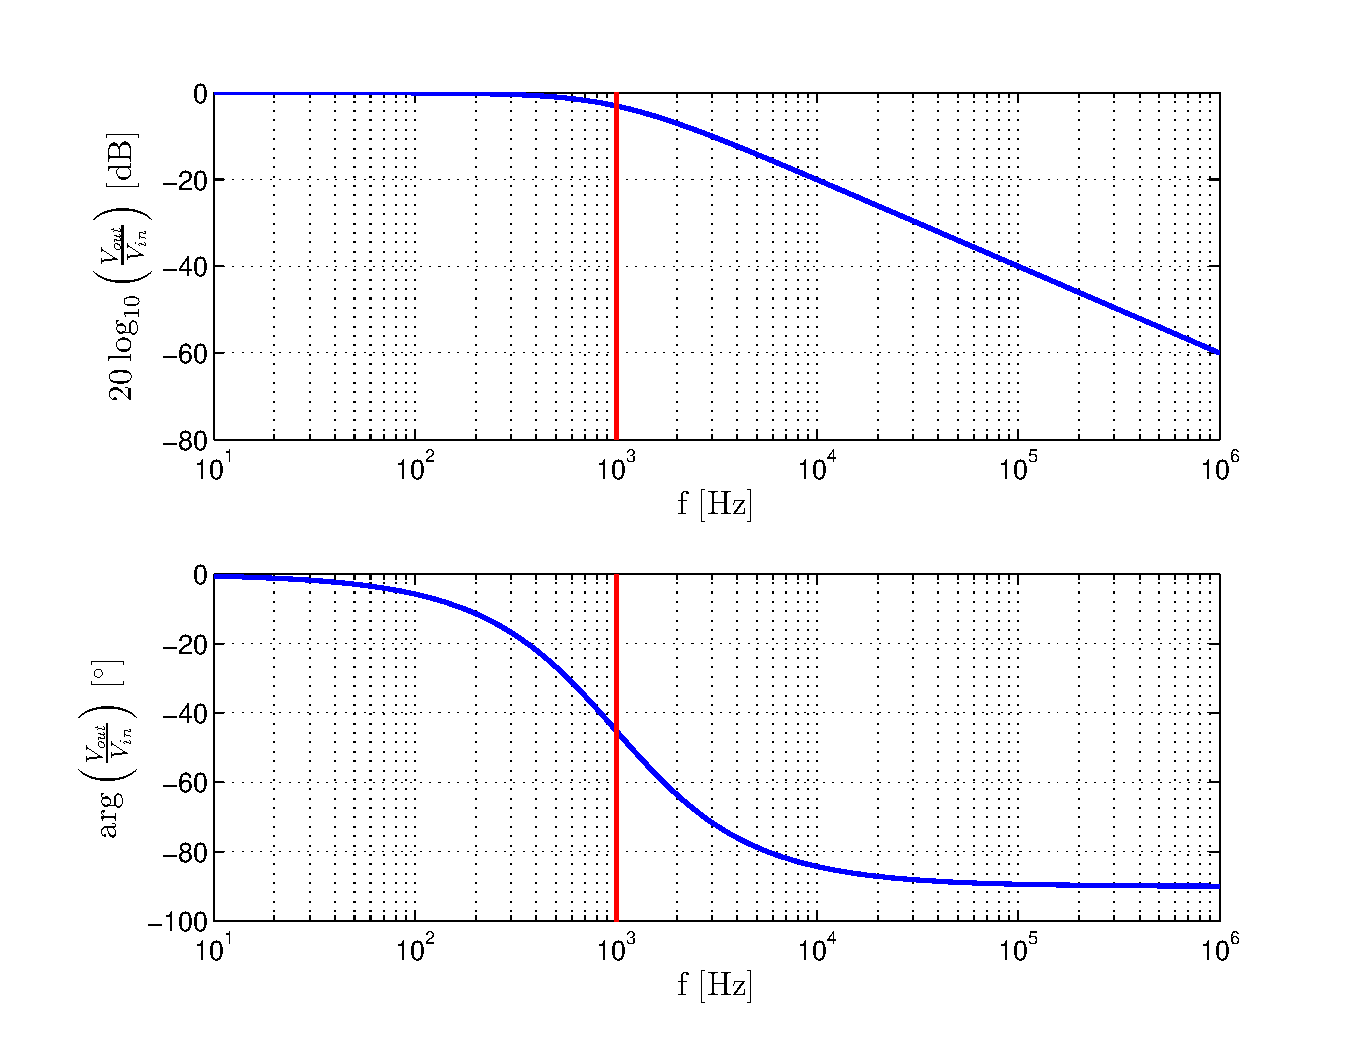
\includegraphics[width=.75\textwidth]{lpf}
	\caption{Diagramme de Bode d'un filtre passe-bas.}
	\label{fig3:lpf}
\end{figure}